%----------------------------------------------------------------------------------------
%	PACKAGES AND THEMES
%----------------------------------------------------------------------------------------
\PassOptionsToPackage{table}{xcolor}
\documentclass[aspectratio=169,xcolor=dvipsnames,svgnames,x11names,fleqn]{beamer}
% \documentclass[aspectratio=169,xcolor=dvipsnames,fleqn]{beamer}

\usetheme{RedVelvet}

\usefonttheme[onlymath]{serif}
\newcommand{\showanswers}{yes}


\usepackage{xspace}
\usepackage{amsmath}
\usepackage{amssymb}
\usepackage{amsfonts}
\usepackage{color}
\usepackage{physics}
% \usepackage{mathbb}
\usepackage{rahul_math}
\usepackage{bigints}

\usepackage{graphicx} % Allows including images
\usepackage{booktabs} % Allows the use of \toprule, \midrule and \bottomrule in tables
\usepackage{tikz,pgfplots}

\usepackage{subfigure}
\usetikzlibrary{arrows}
\usepackage{minted}
\definecolor{LightGray}{gray}{0.9}
\definecolor{cream}{rgb}{0.92, 0.9, 0.55}
\definecolor{lightblue}{rgb}{0.68, 0.85, 0.9}


\usepackage{xcolor-material}
\usetikzlibrary{fit}
\usetikzlibrary{matrix}
\tikzset{%
apple/.pic={
    \fill [MaterialBrown] (-1/8,0)  arc (180:120:1 and 3/2) coordinate [pos=3/5] (@)-- ++(1/6,-1/7)  arc (120:180:5/4 and 3/2) -- cycle;
    \fill [MaterialLightGreen500] (0,-9/10)  .. controls ++(180:1/8) and ++(  0:1/4) .. (-1/3,  -1) .. controls ++(180:1/3) and ++(270:1/2) .. (  -1,   0) .. controls ++( 90:1/3) and ++(180:1/3) .. (-1/2, 3/4) .. controls ++(  0:1/8) and ++(135:1/8) .. (   0, 4/7)
    }
    }

\newcommand{\leftdoublequote}{\textcolor{blue}{\scalebox{3}{``}}}

\newcommand{\rightdoublequote}{\textcolor{blue}{\scalebox{3}{''}}}


\usepackage{textcomp}
\usepackage{fontawesome}
\usepackage{tikz,pgfplots}
\usetikzlibrary{shapes.callouts}
\usetikzlibrary{arrows}
\usetikzlibrary{shapes.geometric, positioning}
\pgfplotsset{compat=1.8} % or newest version

\usetikzlibrary{positioning}


\usepackage{bm}
\usepackage{relsize}



\tikzset{basic/.style={draw,fill=MediumBlue!20,text width=1em,text badly centered}}
\tikzset{input/.style={basic,circle}}
\tikzset{weights/.style={basic,rectangle}}
\tikzset{functions/.style={basic,circle,fill=MediumBlue!10}}



\usepackage{listofitems} % for \readlist to create arrays
\tikzstyle{mynode}=[thick,draw=MediumBlue,fill=MediumBlue!20,circle,minimum size=22]


\usepackage{overpic}

%----------------------------------------------------------------------------------------
%	TITLE PAGE
%----------------------------------------------------------------------------------------

\usepackage{tikz-qtree,tikz-qtree-compat}
\usetikzlibrary{tikzmark}
\usetikzlibrary{calc}

\usetikzlibrary{fit}
\tikzset{%
apple/.pic={
    \fill [MaterialBrown] (-1/8,0)  arc (180:120:1 and 3/2) coordinate [pos=3/5] (@)-- ++(1/6,-1/7)  arc (120:180:5/4 and 3/2) -- cycle;
    \fill [MaterialLightGreen500] (0,-9/10)  .. controls ++(180:1/8) and ++(  0:1/4) .. (-1/3,  -1) .. controls ++(180:1/3) and ++(270:1/2) .. (  -1,   0) .. controls ++( 90:1/3) and ++(180:1/3) .. (-1/2, 3/4) .. controls ++(  0:1/8) and ++(135:1/8) .. (   0, 4/7)
}
}
\usepackage{tikz-qtree,tikz-qtree-compat}
\usetikzlibrary{tikzmark}
\usetikzlibrary{calc}




\title[CPE 486/586: Machine Learning]{CPE 486/586: Machine Learning for Engineers} % The short title appears at the bottom of every slide, the full title is only on the title page
\subtitle{13 Neural Network}

\author[Rahul Bhadani] {{\Large \textbf{Rahul Bhadani}}}

\institute[UAH] % Your institution as it will appear on the bottom of every slide, maybe shorthand to save space
{
    Electrical \& Computer Engineering,  The University of Alabama in Huntsville
}
\date

% \titlegraphic{
%    \includegraphics[width=0.4\linewidth]{figures/UAH_primary.png}
% }

\begin{document}

%-------------------------------------------------
\begin{frame}
    \titlepage
\end{frame}

%-------------------------------------------------
\begin{frame}{Outline}
    \backgroundtableofcontents
\end{frame}






\begin{sectionframe}{\faChild}{Motivation}
\end{sectionframe}


%------------------------------------------------
\begin{frame}{Lecture Overview}
    \begin{itemize}
        \item Our goal is to develop an understanding of how neural networks work and how they can be trained. 
        \item Neural networks are universal approximators. The universal approximation theorem implies that neural networks can represent a wide variety of functions when given appropriate weights. They typically do not provide a construction for the weights, but merely state that such a construction is possible.
    \end{itemize}
\end{frame}



\begin{sectionframe}{\faFa}{A Brief History of Neural Networks}
\end{sectionframe}





%------------------------------------------------
\begin{frame}{A Brief History of Neural Networks}


\begin{columns}
%------------------------------------------------
\column{.45\textwidth}
\begin{tblock}{Perceptron}
\begin{itemize}
    \item The percepton is the first single layer network that has an ``artificial'' neuron, which was developed by Frank Rozenblat (1957). 
    \item Designed for binary classification tasks. 
    \item Optimization does not converge for nonlinearly separable datasets. 
\end{itemize}
\end{tblock}
%------------------------------------------------
\column{.45\textwidth}
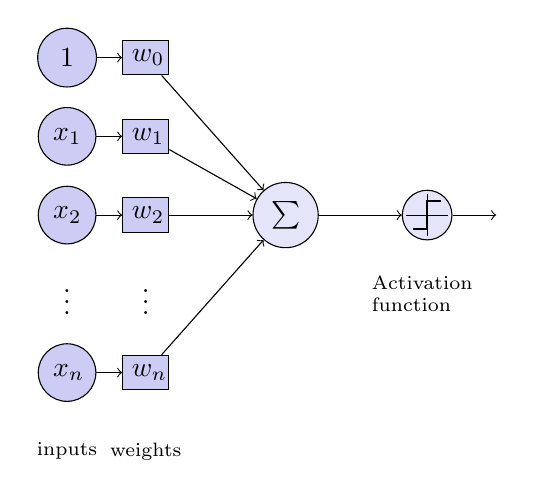
\begin{tikzpicture}
        \node[functions] (center) {};
        \node[below of=center,font=\scriptsize,text width=4em] {Activation function};
        \draw[thick] (0.5em,0.5em) -- (0,0.5em) -- (0,-0.5em) -- (-0.5em,-0.5em);
        \draw (0em,0.75em) -- (0em,-0.75em);
        \draw (0.75em,0em) -- (-0.75em,0em);
        \node[right of=center] (right) {};
            \path[draw,->] (center) -- (right);
        \node[functions,left=3em of center] (left) {$\sum$};
            \path[draw,->] (left) -- (center);
        \node[weights,left=3em of left] (2) {$w_2$} -- (2) node[input,left of=2] (l2) {$x_2$};
            \path[draw,->] (l2) -- (2);
            \path[draw,->] (2) -- (left);
        \node[below of=2] (dots) {$\vdots$} -- (dots) node[left of=dots] (ldots) {$\vdots$};
        \node[weights,below of=dots] (n) {$w_n$} -- (n) node[input,left of=n] (ln) {$x_n$};
            \path[draw,->] (ln) -- (n);
            \path[draw,->] (n) -- (left);
        \node[weights,above of=2] (1) {$w_1$} -- (1) node[input,left of=1] (l1) {$x_1$};
            \path[draw,->] (l1) -- (1);
            \path[draw,->] (1) -- (left);
        \node[weights,above of=1] (0) {$w_0$} -- (0) node[input,left of=0] (l0) {$1$};
            \path[draw,->] (l0) -- (0);
            \path[draw,->] (0) -- (left);
        \node[below of=ln,font=\scriptsize] {inputs};
        \node[below of=n,font=\scriptsize] {weights};
\end{tikzpicture}

\end{columns}


\end{frame}




%------------------------------------------------
\begin{frame}{A Brief History of Neural Networks}


\begin{columns}
%------------------------------------------------
\column{.5\textwidth}
\begin{tblock}{Minsky \& Papert (1969)}
\begin{itemize}
    \item Minsky \& Papert published a work that was the ``kiss of death'' for neural network research.
    \item Claim: Perceptrons cannot solve the XOR problem (arguably the easiest nonlinear task)! 
    \item Neural network research came to a halt for nearly 15 years.
\end{itemize}
\end{tblock}
%------------------------------------------------
\column{.5\textwidth}
\begin{center}
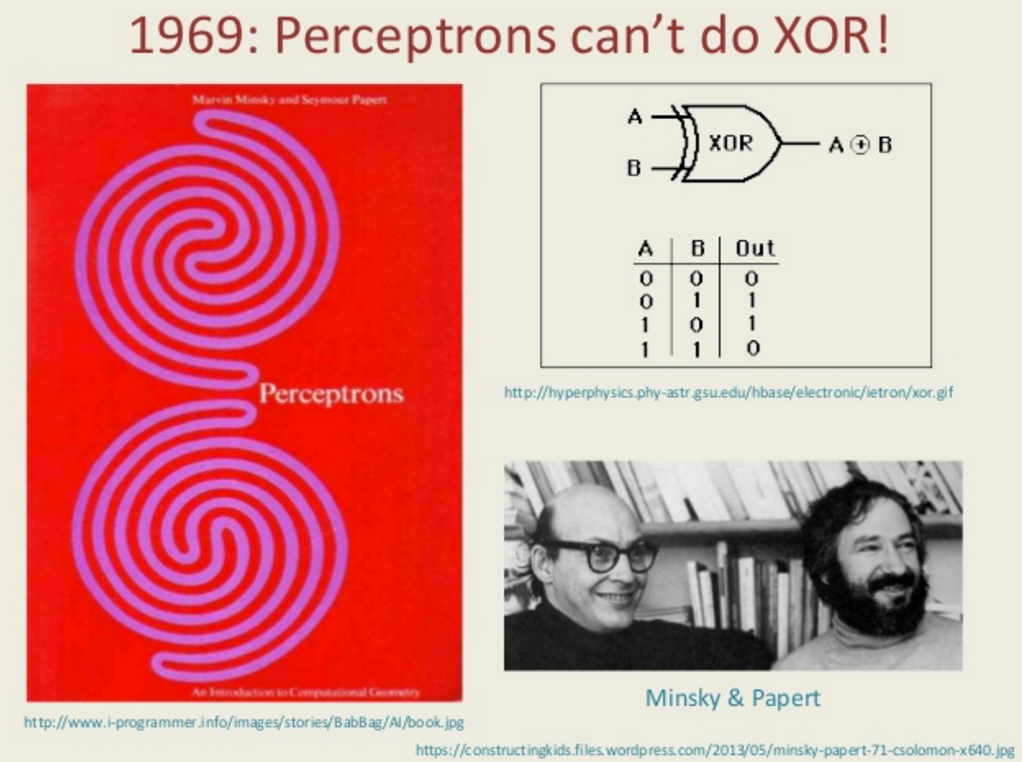
\includegraphics[width=.9\textwidth]{figures/ml-xor.png}
\end{center}
\end{columns}

\end{frame}





%------------------------------------------------
\begin{frame}{A Brief History of Neural Networks}

\vspace{5pt}
\begin{columns}
%------------------------------------------------
\column{.65\textwidth}
\begin{tblock}{Backpropagation }
\begin{itemize}
    \item Werbos (1974), Rummelhart and Hinton (1986) were major contributors to the backpropagation algorithm, which is how we train neural networks. 
    \item Werbos' 1974 PhD thesis from Harvard University presented the backpropagation algorithm. It wasn't until the 1980's that neural network research picked back up. 
    \item Backprop even goes back to Kelley's work in 1960 on continuous-time control theory. 
\end{itemize}
\end{tblock}
%------------------------------------------------
\column{.35\textwidth}
\begin{center}
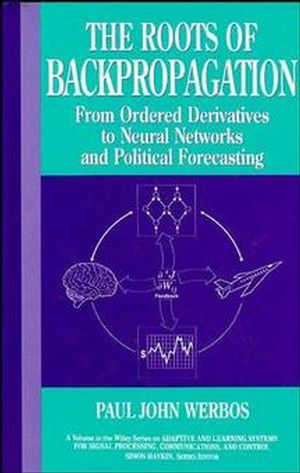
\includegraphics[width=.6\textwidth]{figures/nn-backprop.jpg}
\end{center}

\end{columns}


\end{frame}





\begin{sectionframe}{\faCubes}{The Multilayer Perceptron and Backpropagation}
\end{sectionframe}





%------------------------------------------------
\begin{frame}{Definitions}

\begin{tblock}{From Microsoft Encarta}
A neural network is a highly interconnected network of information-processing elements that mimics the connectivity and functioning of the human brain. One of the most significant strengths of neural networks is their ability to learn from a limited set of examples.
\end{tblock}

\end{frame}


%------------------------------------------------
\begin{frame}{A Neural Network}

\begin{center}
    
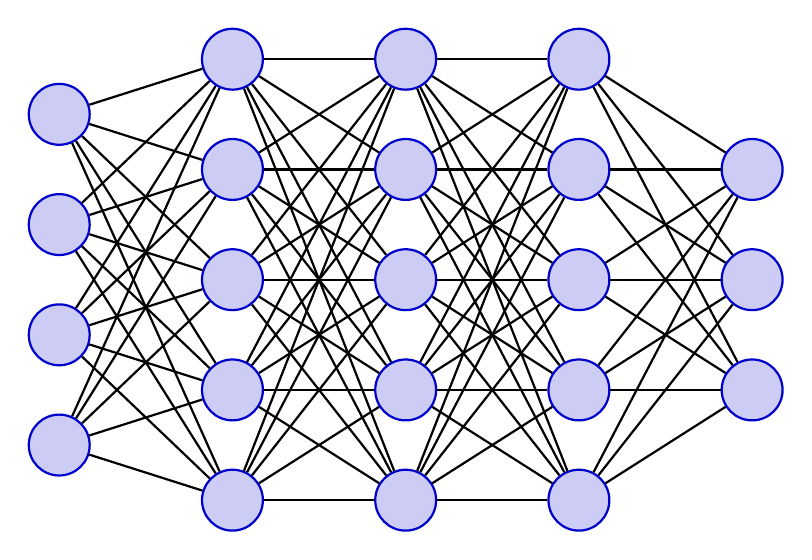
\begin{tikzpicture}[x=2.2cm,y=1.4cm]
  \readlist\Nnod{4,5,5,5,3} % number of nodes per layer
  % \Nnodlen = length of \Nnod (i.e. total number of layers)
  % \Nnod[1] = element (number of nodes) at index 1
  \foreachitem \N \in \Nnod{ % loop over layers
    % \N     = current element in this iteration (i.e. number of nodes for this layer)
    % \Ncnt  = index of current layer in this iteration
    \foreach \i [evaluate={\x=\Ncnt; \y=\N/2-\i+0.5; \prev=int(\Ncnt-1);}] in {1,...,\N}{ % loop over nodes
      \node[mynode] (N\Ncnt-\i) at (\x,\y) {};
      \ifnum\Ncnt>1 % connect to previous layer
        \foreach \j in {1,...,\Nnod[\prev]}{ % loop over nodes in previous layer
          \draw[thick] (N\prev-\j) -- (N\Ncnt-\i); % connect arrows directly
        }
      \fi % else: nothing to connect first layer
    }
  }
\end{tikzpicture}
\end{center}

\end{frame}




%------------------------------------------------
%------------------------------------------------
\begin{frame}{A Tour of Neural Networks}
\begin{center}
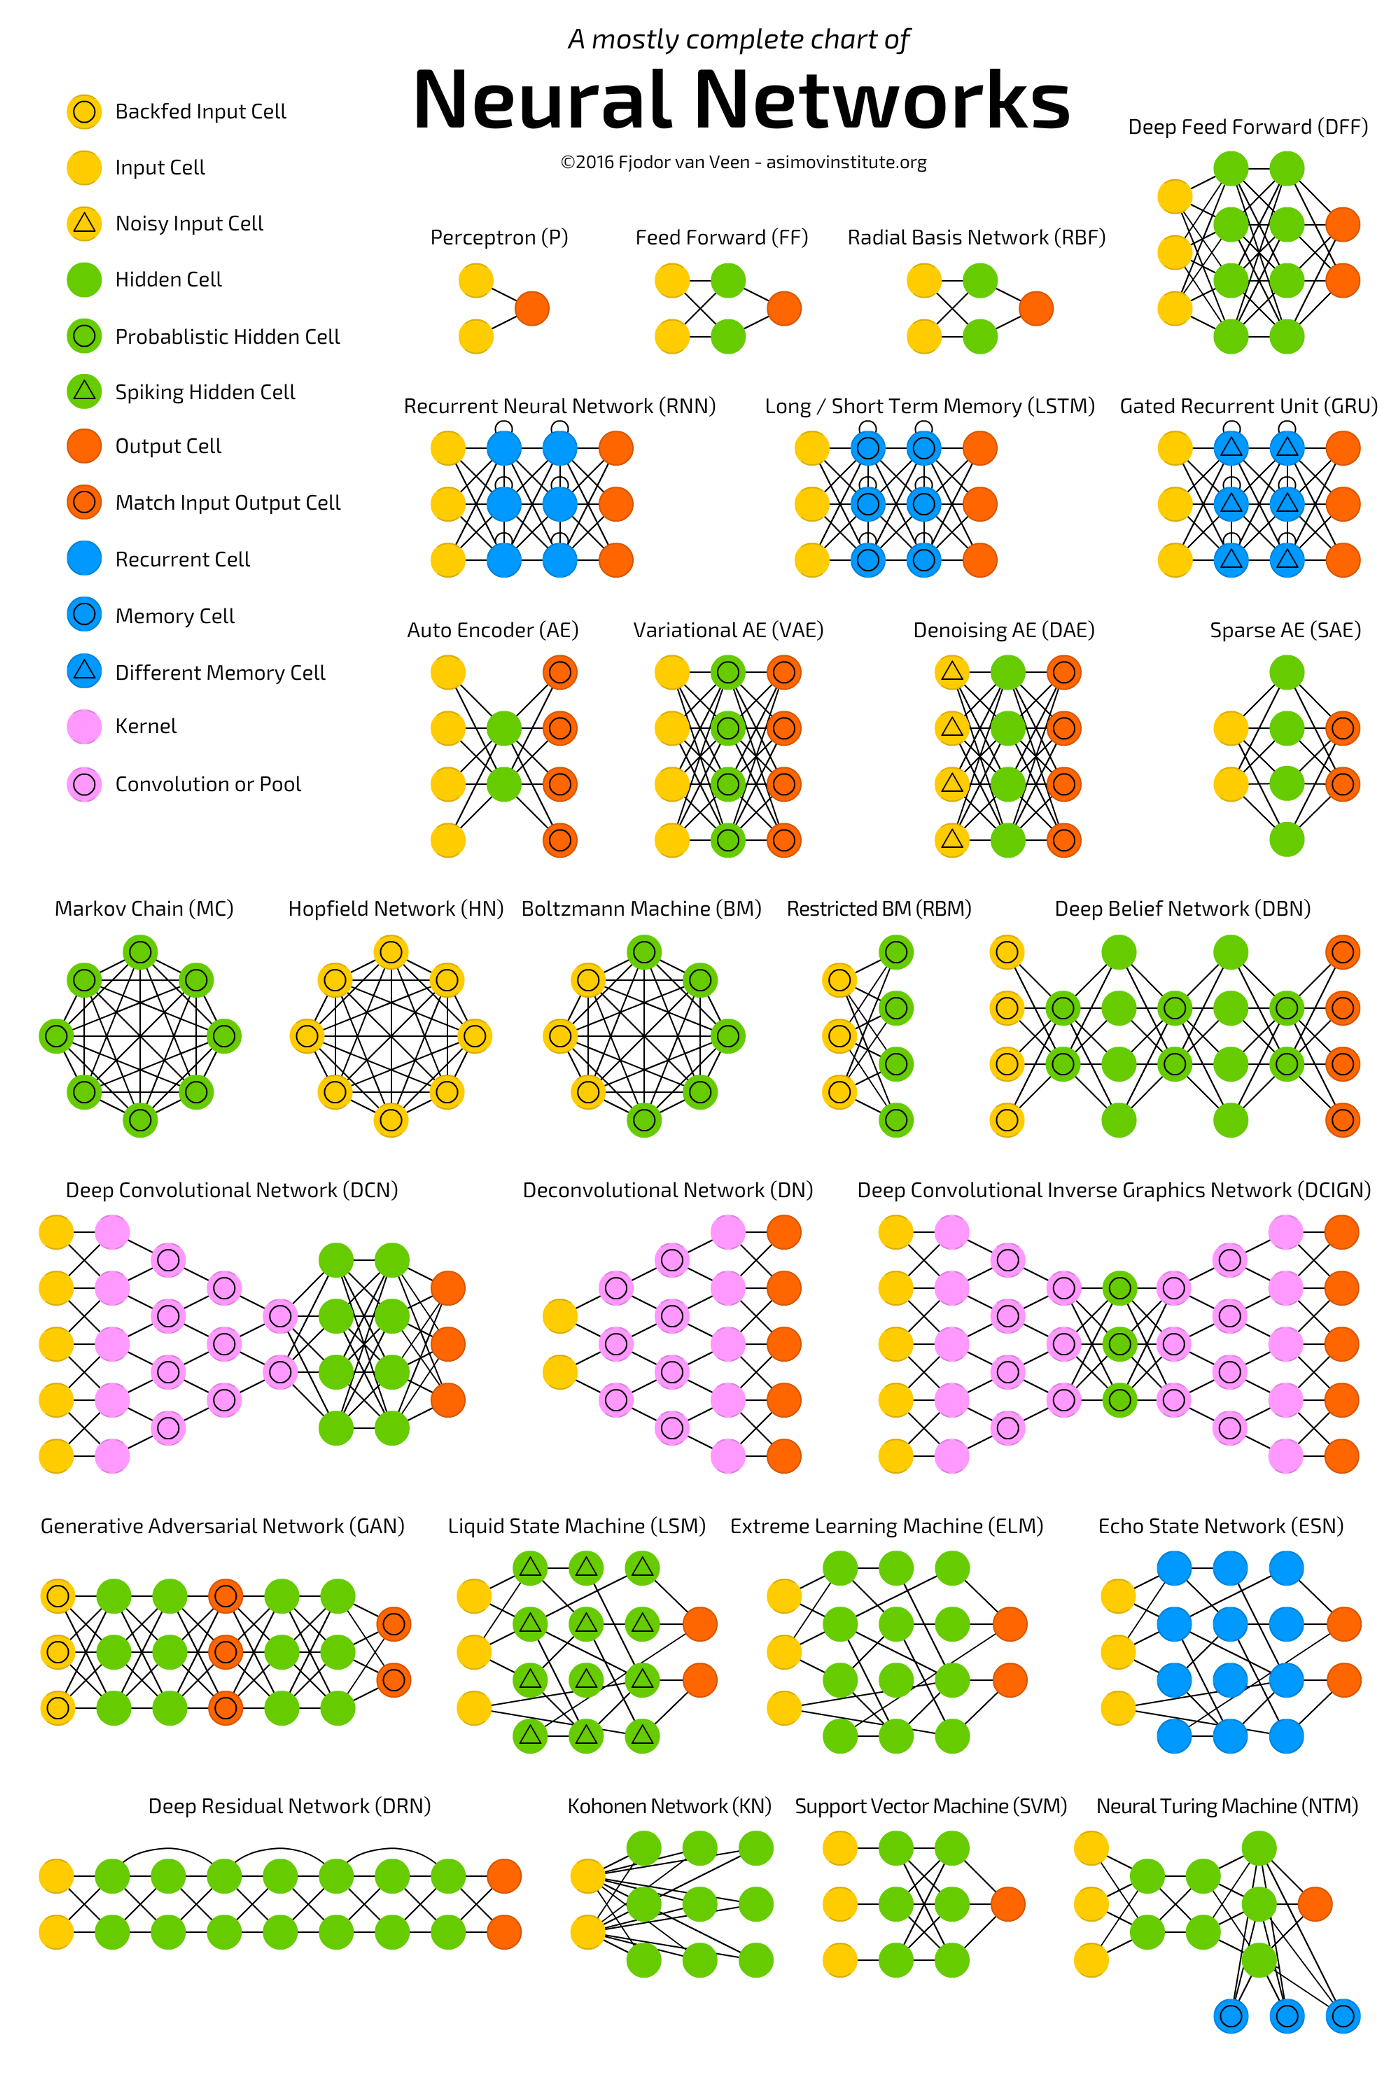
\includegraphics[height=.75\textheight]{figures/nns.png}
\end{center}
\end{frame}


%------------------------------------------------
\begin{frame}{Definitions}
\begin{itemize}
    \item We assume a supervised learning setting where we're provided a training data set $\Dcal:= \{\xbf(n), \dbf(n)\}_{n=1}^N$, where $\x(n)$ is a feature vector and $\dbf(n)$ is the desired output for the $n$th sample.
    \begin{itemize}
        \item Notation such as $d_j(n)$ is used to refer to the $j$th output node of the desired signal
        \item Neuron and node are used interchangeably 
    \end{itemize}
    \item The first and last layers of the network are referred to as the input and output layer, respectively. All layers between the input and output are referred to as {\em hidden layers}. 
    \item For the moment, we're only going to exam a neural network with one hidden layer; however, we can generalize the results to multiple hidden layers. 
    \begin{itemize}
        \item Training a very deep network can be challenging due to issues we cover in this lecture and future lectures will address training a deep network. 
    \end{itemize}
\end{itemize}
\end{frame}


%------------------------------------------------
\begin{frame}{An Example}
\begin{talert}{The Credit Assignment Problem}
\begin{itemize}
    \item The {\color{MediumBlue}credit assignment problem} is one where we seek to credit or blame for overall outcomes to each of the internal decisions made by the hidden computational units. 
    \begin{itemize}
        \item These hidden units are the first to ``blame'' for an error made at the output because the data are processed internally before ever reaching the output. 
        \item How much ``weight'' or ``credit'' do we assign a neuron when an error is made at the output? 
    \end{itemize}
    \item The {\em \color{MediumRed}backpropagation algorithm} solves the credit assignment problem in an elegant manner. 
\end{itemize}
\end{talert}
\end{frame}




% \begin{center}
% 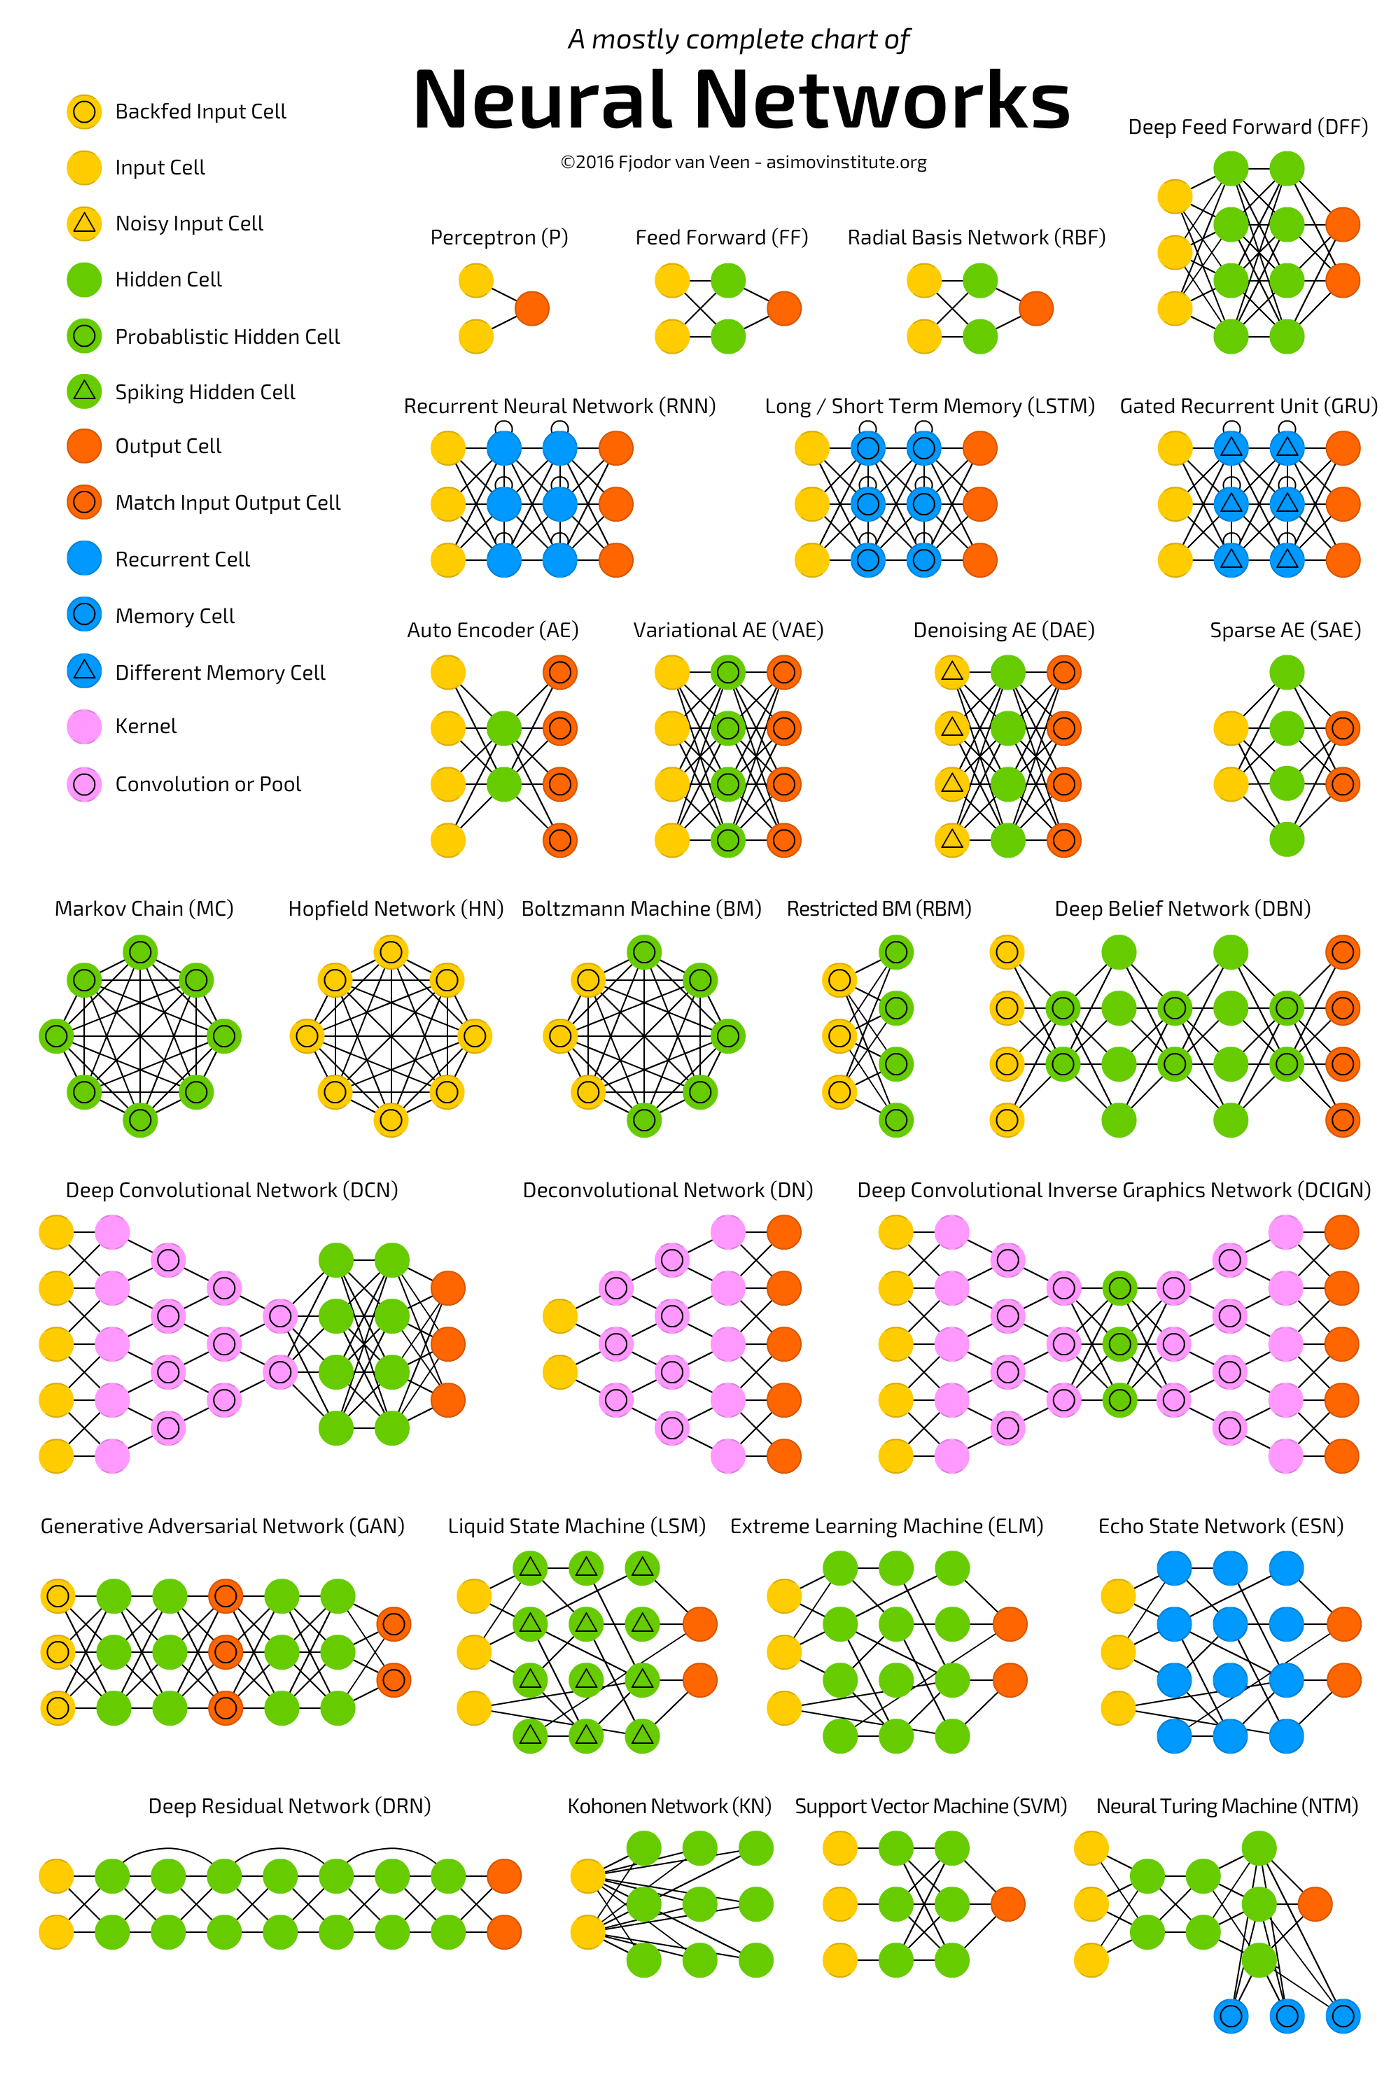
\includegraphics[height=.85\textheight]{figures/nns.png}
% \end{center}


\begin{sectionframe}{\faQuestionCircle}{Setting up the Problem}
\end{sectionframe}




%------------------------------------------------
\begin{frame}{Defining the error}

\begin{tblock}{}
A data $\x(n)$ is passed through the network and the measured output of the neural network is $\ybf(n)$. \uncover<2->{The error signal, $e_j(n)$}\uncover<3->{, instantaneous error energy, $E_j(n)$}\uncover<4->{, and total error, $E(n)$, is given by:}
\vspace{-1em}
\begin{multiequation}
\uncover<2->{e_j(n) = d_j(n) - y_j(n),} \hspace{1em}
\uncover<3->{E_j(n) = \frac{1}{2}e_j^2(n),} \hspace{1em}
\uncover<4->{E(n) = \sum_{j=1}^C E_j(n) = \frac{1}{2}\sum_{j=1}^C e_j^2(n)}
\end{multiequation}
%\uncover<4->{where we denoted $E(n)$ and $e_j(n)$ as EQ01 and EQ02, respectively. }
\end{tblock}
\end{frame}

\begin{frame}{The Total Error Overall Samples}
	\begin{cotton}{}
		\begin{multiequation}
		E_{av}(N) = \frac{1}{N} \sum_{n=1}^N E(n) = \frac{1}{2N}\sum_{n=1}^{N}\sum_{j=1}^C e_j^2(n)
		\end{multiequation}
		\end{cotton}
\end{frame}





%------------------------------------------------
\begin{frame}{Signal Flow at a Neuron}

\begin{center}
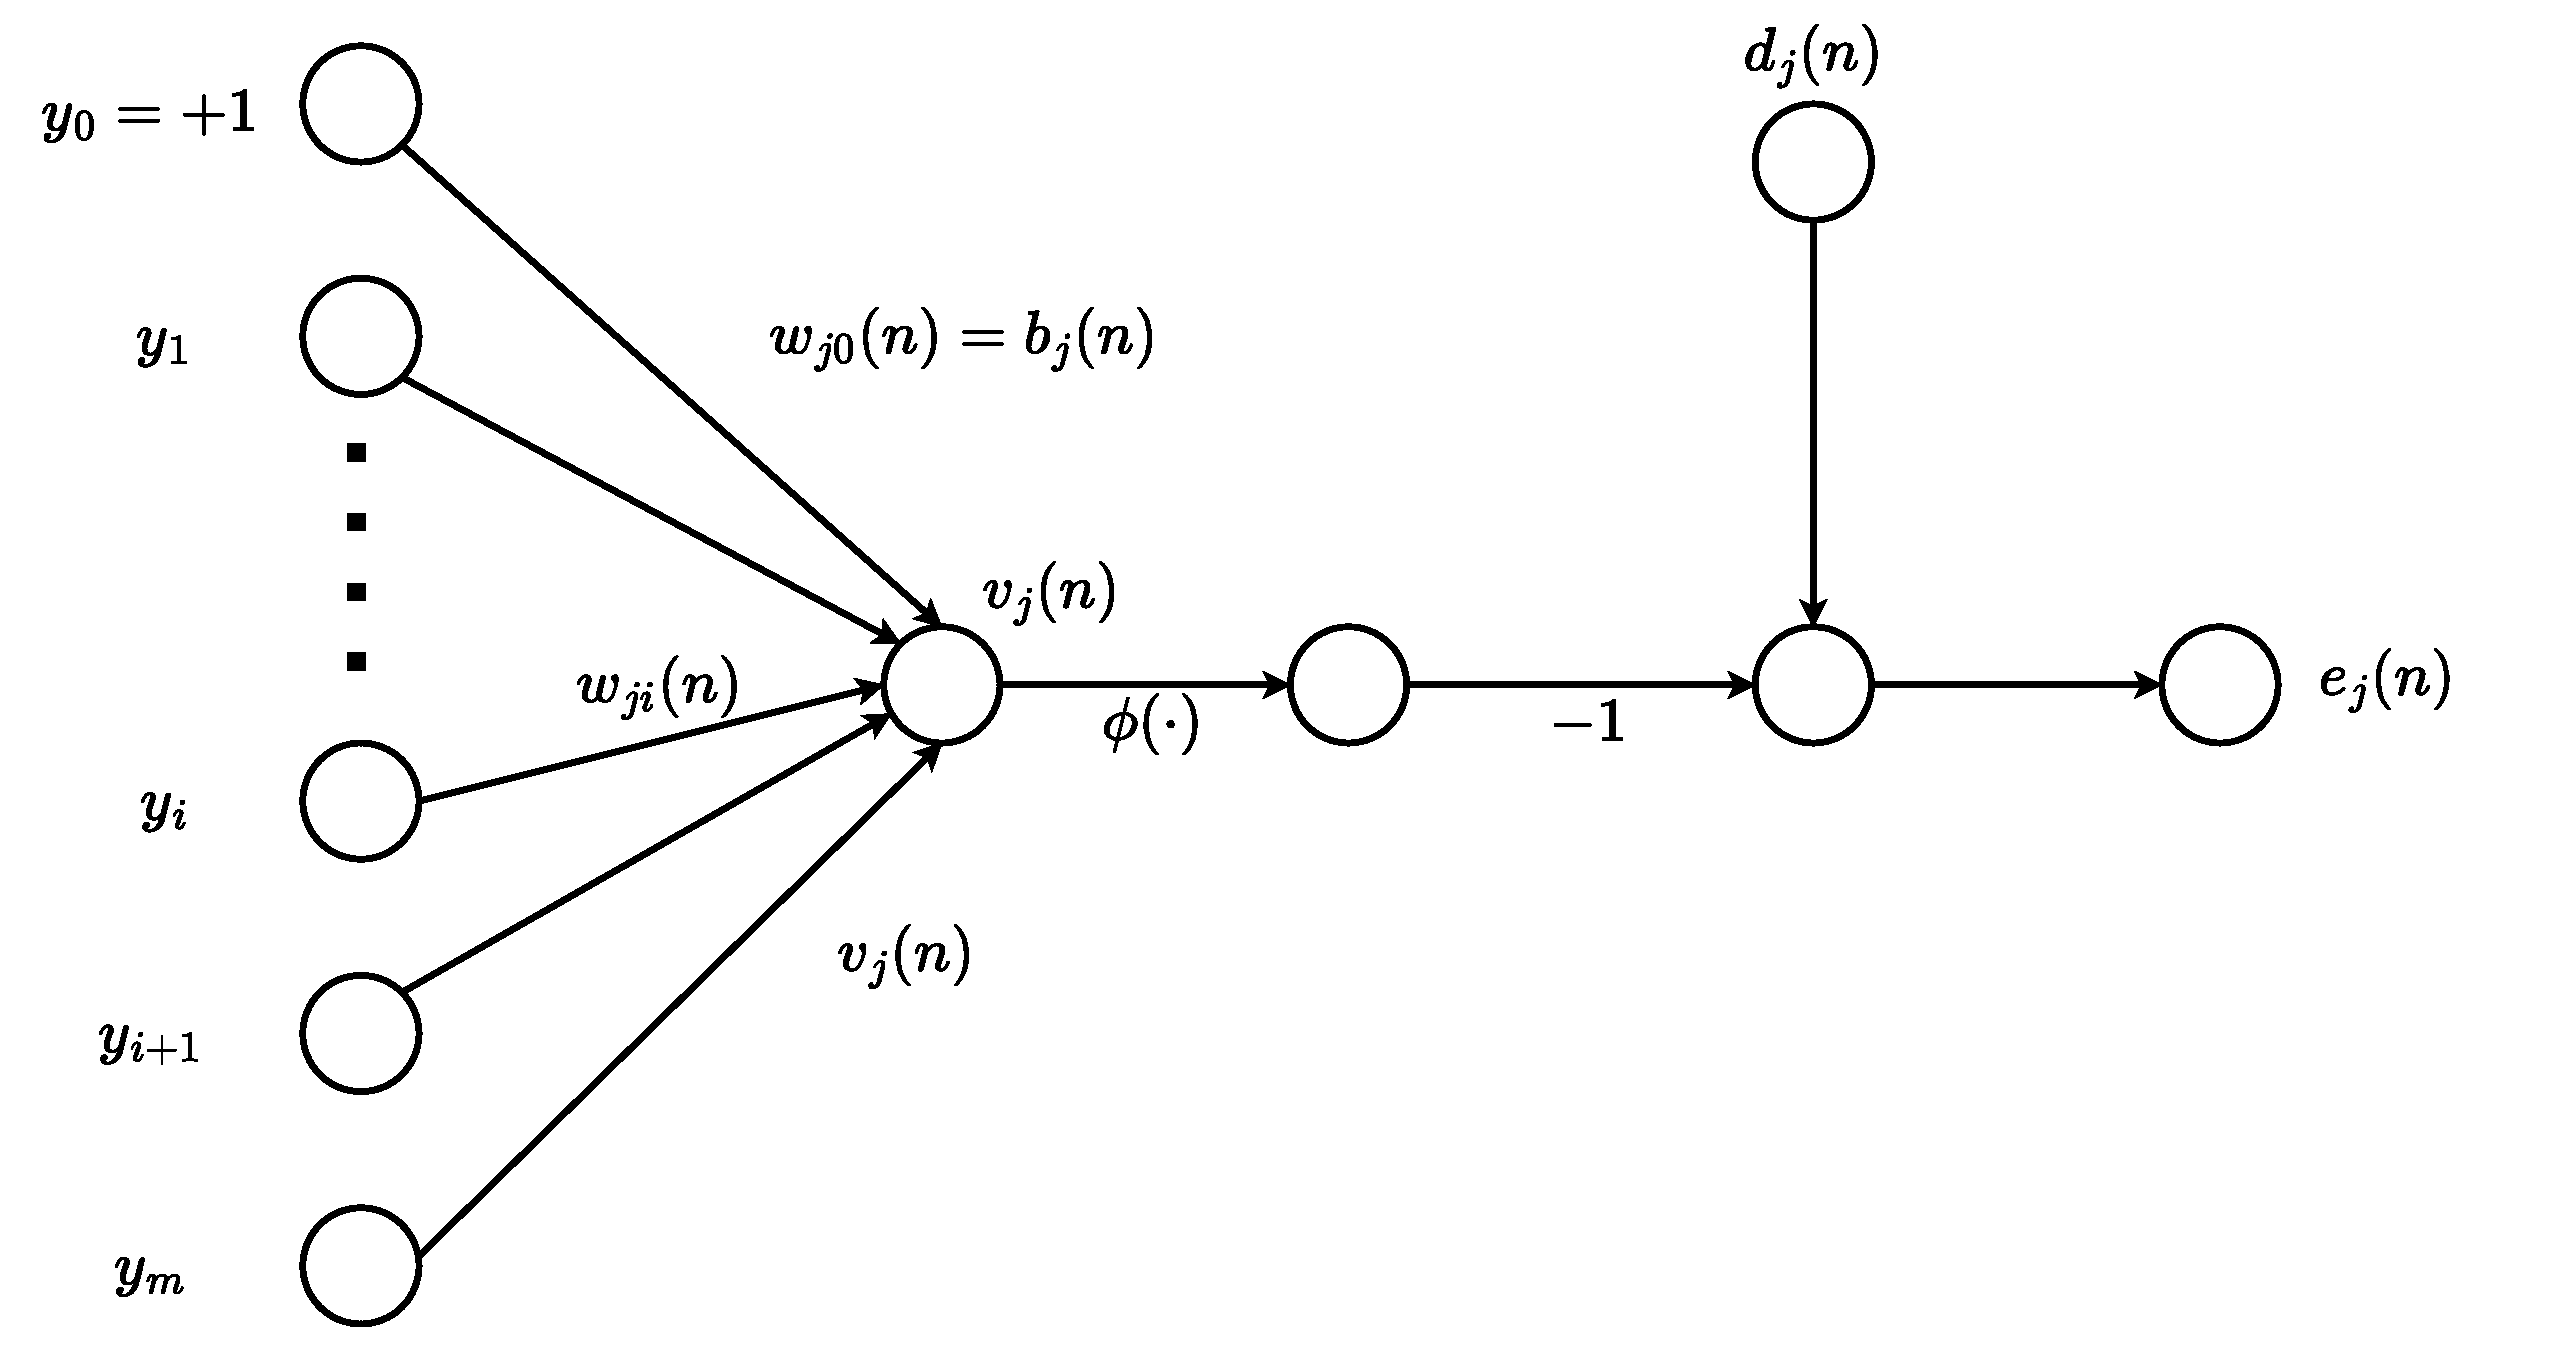
\includegraphics[width=.8\textwidth]{figures/nn-signal-flow.pdf}
\end{center}
\end{frame}



%------------------------------------------------
\begin{frame}{Signal Flow at a Neuron}
\begin{twilight}{}
The {\em induced local field}, $v_j(n)$ is produced at the input of the activation associated with neuron $j$, which is given by: 
\begin{multiequation}
    v_j(n) = \sum_{i=1}^m w_{ji}(n) y_i(n)
\end{multiequation}
\uncover<2->{
The signal at the neuron is 
\begin{multiequation}
    y_j(n) = \phi(v_j(n))
\end{multiequation}
where $\phi(\cdot)$ is a nonlinear {\em activation function}. We refer to $y_j(n)$ and $v_j(n)$ as EQ3 and EQ4, respectively. 
}
\end{twilight}
\end{frame}



%------------------------------------------------
\begin{frame}{Example Activation Functions}
\begin{center}
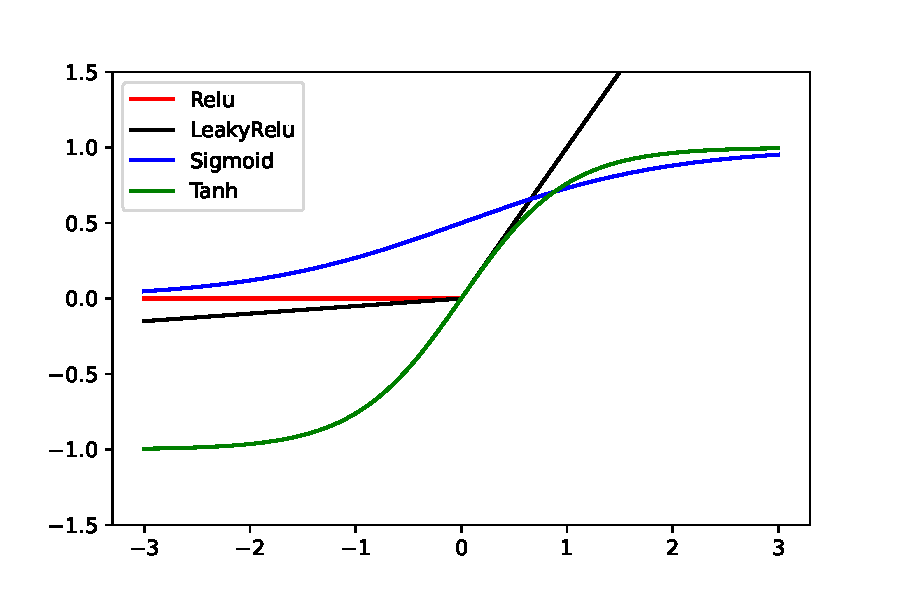
\includegraphics[width=.65\textwidth]{figures/nn-activation.pdf}
\end{center}
\end{frame}




%------------------------------------------------
\begin{frame}{Setting up gradient descent}
\begin{tblock}{Keeping our eye on the prize}
Out goal is to determine the update rule for the weights of the neural network using gradient descent. Therefore, we need to find the gradient of the error w.r.t. the parameters $\wbf$. Recall that the update for gradient descent is given by: 
\begin{multiequation}
\wbf(t+1) = \wbf(t) + \Delta\wbf(t) = \wbf(t) -\eta \frac{\partial E}{\partial\wbf}
\end{multiequation}
\end{tblock}


\end{frame}

\begin{frame}{Finding the Gradient is Challenging}
	\begin{talert}{}
		The term $\wbf$ does not show up in the expression for $E$, which makes finding $\frac{\partial E}{\partial\wbf}$ more challenging. Finding the gradient is going to be very difficult unless we look at the problem differently. 
		\end{talert}
\end{frame}



%------------------------------------------------
\begin{frame}{Back to the basics of calculus}

\begin{tblock}{Calculus 101: The Chain Rule}
We need to find an expression for ${\partial E(n)}/{\partial w_{ji}(n)}$. One way to find this expression is to use the chain rule of calculus. The partial ${\partial E(n)}/{\partial w_{ji}(n)}$ represents the {\em sensitivity factor} that determines the direction of the search weight space for the synaptic weight $w_{ji}(n)$.  
\begin{multiequation}
\frac{\partial E(n)}{\partial w_{ji}(n)} = 
\frac{\partial E(n)}{\partial e_{j}(n)} \cdot 
\frac{\partial e_j(n)}{\partial y_{j}(n)} \cdot 
\frac{\partial y_j(n)}{\partial v_{j}(n)} \cdot 
\frac{\partial v_j(n)}{\partial w_{ji}(n)}
\end{multiequation}
\end{tblock}



\end{frame}



\begin{frame}{}

	\begin{tblock}{}
		Our goal is to work with derivatives above to find the gradient updates when we're at an output neuron. 
	\end{tblock}

	
\end{frame}
%------------------------------------------------
\begin{frame}{Filling in the Missing Pieces of ${\partial E(n)}/{\partial w_{ji}(n)}$}


	\begin{center}
		\begin{tblock}{}
			\begin{multiequation}
				E(n) & = \frac{1}{2}\sum e_j^2(n)\\
				\frac{\partial E(n)}{\partial e_j(n)} & = e_j(n)
			\end{multiequation}
			\end{tblock}
	\end{center}

\end{frame}

%

%------------------------------------------------
\begin{frame}{Filling in the Missing Pieces of ${\partial E(n)}/{\partial w_{ji}(n)}$}


	\begin{center}
		\begin{tblock}{}
			\begin{multiequation}
				e_j(n) & = d_j(n) - y_j(n)\\
				\frac{\partial e_j(n)}{\partial y_j(n)} & = -1
			\end{multiequation}
		\end{tblock}
	\end{center}

\end{frame}
%


%------------------------------------------------
\begin{frame}{Filling in the Missing Pieces of ${\partial E(n)}/{\partial w_{ji}(n)}$}


	\begin{center}
		\begin{block}{$y_j(n) = \phi(v_j(n))$}
			\begin{multiequation}
				\frac{\partial y_j(n)}{\partial v_j(n)} = \phi'(v_j(n))
			\end{multiequation}
			\end{block}
	\end{center}

\end{frame}



%------------------------------------------------
\begin{frame}{Filling in the Missing Pieces of ${\partial E(n)}/{\partial w_{ji}(n)}$}


	\begin{center}
		\begin{block}{$v_j(n) = \sum w_{ji}(n) y_i(n)$}
			\begin{multiequation}
				\frac{\partial v_j(n)}{\partial w_{ji}(n)} = y_i(n)
			\end{multiequation}
			\end{block}
	\end{center}

\end{frame}


%------------------------------------------------
\begin{frame}{Filling in the Missing Pieces of ${\partial E(n)}/{\partial w_{ji}(n)}$}


	\begin{center}
		\begin{exampleblock}{Putting it all together}
			\begin{multiequation}
			\frac{\partial E(n)}{\partial w_{ji}(n)} = 
			\frac{\partial E(n)}{\partial e_{j}(n)} \cdot 
			\frac{\partial e_j(n)}{\partial y_{j}(n)} \cdot 
			\frac{\partial y_j(n)}{\partial v_{j}(n)} \cdot 
			\frac{\partial v_j(n)}{\partial w_{ji}(n)} = - e_j(n) \phi'(v_j(n)) y_i(n)
			\end{multiequation}
			\end{exampleblock}
	\end{center}

\end{frame}




%------------------------------------------------
\begin{frame}{The Local Gradient}

\begin{exampleblock}{Definition}
We're going to define new term that will be useful for the rest of the discussion on backpropagation. The {\em local gradient} at neuron $j$ is given by:  
\begin{multiequation}
\delta_j(n) = \frac{\partial E(n)}{\partial v_j(n)} = e_j(n) \phi'(v_j(n))
\end{multiequation}
\end{exampleblock}


\end{frame}





%------------------------------------------------
\begin{frame}{The Local Gradient}


\begin{block}{Case 1: Neuron $j$ is an output node}
When neuron $j$ is located in the output layer of the network, it is supplied with a desired response. We can use EQ1 to compute the error $e_j(n)$ associated with this neuron. Having determined $e_j(n)$ we can easily calculate the local gradient $\delta_j(n)$. 
\end{block}

\uncover<2->{
\begin{block}{Case 2: Neuron $j$ is a hidden node}
When neuron $j$ is located in the hidden layer of the network, there is not a desired response. The error signal for a hidden neuron would have to be determined recursively and working backwards in terms of the error of all the neurons to which that hidden neuron is directly connected. {\em \color{MediumRed} This is where backpropogation gets interesting!}
\end{block}
}

\end{frame}






%------------------------------------------------
\begin{frame}{Redefining the Local Gradient}

\begin{tblock}{New definitions of the local gradient and error at the output}
Let $j$ denote a neuron at a hidden layer (i.e., $j$ is no longer used for an arbitrary neuron). Then the local gradient at hidden neuron $j$ is given by 
\begin{multiequation}
\delta_j(n) = - \frac{\partial E(n)}{\partial y_j(n)}
\cdot \frac{\partial y_j(n)}{\partial v_j(n)}
= - \frac{\partial E(n)}{\partial y_j(n)} \cdot \phi'(v_j(n))
\end{multiequation}
\uncover<2->{
The error gradient at this neuron is given by $\frac{\partial E(n)}{\partial y_j(n)}$ and we now use $k$ to denote neurons at the output layer. }
\begin{multiequation}
\uncover<2->{E(n)  = \frac{1}{2}\sum_{k=1}^C e_k^2(n), }\hspace{2em}
\uncover<3->{
\frac{\partial E(n)}{\partial y_j(n)} = \sum_{k=1}^C e_k(n) \frac{\partial e_k(n)}{\partial y_j(n)}
}
\uncover<4->{
= \sum_{k=1}^C e_k(n) \frac{\partial e_k(n)}{\partial v_k(n)} \frac{\partial v_k(n)}{\partial y_j(n)}
}
\end{multiequation}
\end{tblock}


\end{frame}



%------------------------------------------------
\begin{frame}{Filling in the missing pieces}
\begin{tblock}{}
\begin{multiequation}
\frac{\partial E(n)}{\partial y_j(n)} 
= \sum_{k=1}^C e_k(n) \frac{\partial e_k(n)}{\partial v_k(n)} \frac{\partial v_k(n)}{\partial y_j(n)}
\uncover<2->{
=- \sum_{k=1}^C  \underbrace{ e_k(n)  \phi_k(v_k(n))}_{\text{Seen this before? } \delta_k(n) } w_{kj}(n)
}
\end{multiequation}
\end{tblock}


\begin{talert}{}
We have $e_k(n) = d_k(n) - y_k(n)$
\begin{multiequation}
\frac{\partial e_k(n)}{\partial v_k(n)} 
&= \frac{\partial }{\partial v_k(n)}\left\{ d_k(n) - y_k(n)\right\}
= \frac{\partial }{\partial v_k(n)}\left\{ d_k(n) - \phi_k(v_k(n))\right\}
= -\phi_k(v_k(n))
\\
\frac{\partial v_k(n)}{\partial y_j(n)} &= 
\frac{\partial }{\partial y_j(n)} 
\left\{ \sum_{j=1}^m w_{kj}(n) y_j(n) \right\}
= w_{kj}(n)
\end{multiequation}
\end{talert}
\end{frame}


%------------------------------------------------
\begin{frame}{The Local Gradient}

New definition of the local gradient, $\delta_j(n)$

\begin{tblock}{}
Let $j$ denote a neuron at a hidden layer (i.e., $j$ is no longer used for an arbitrary neuron). Then the local gradient at hidden neuron $j$ is given by 
\begin{multiequation}
\delta_j(n) = - \frac{\partial E(n)}{\partial y_j(n)} \cdot \phi'(v_j(n))
= \phi'(v_j(n)) \sum_{k=1}^C \delta_k(n) w_{kj}(n)
\end{multiequation}
\end{tblock}
\end{frame}


\begin{frame}{Update rule for any neuron}
	


\begin{block}{}
	\begin{multiequation}
	\begin{pmatrix}
	\text{weight} \\
	\text{correction} \\
	\Delta w_{ij}(n)
	\end{pmatrix}
	= \eta 
	\begin{pmatrix}
	\text{local} \\
	\text{gradient} \\
	\delta_{j}(n)
	\end{pmatrix}
	\begin{pmatrix}
	\text{Input Signal} \\
	\text{at neuron }i \\
	y_i(n)
	\end{pmatrix}
	\end{multiequation}
	\end{block}

	
\end{frame}



%------------------------------------------------
\begin{frame}{Example: MNIST}
\begin{center}
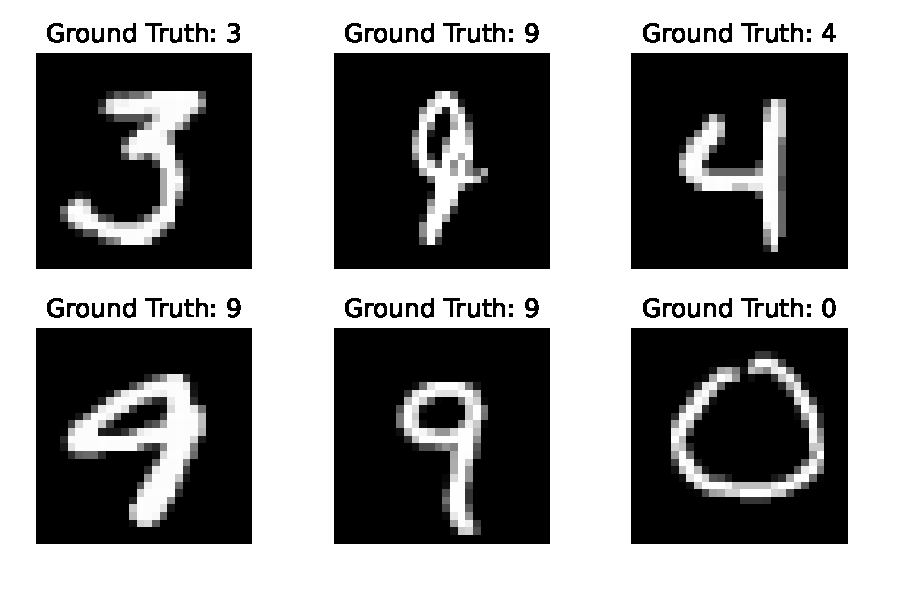
\includegraphics[width=.6\textwidth]{figures/nn-mnist.pdf}
\end{center}
\end{frame}


%------------------------------------------------
\begin{frame}{Example: MNIST}
\begin{center}
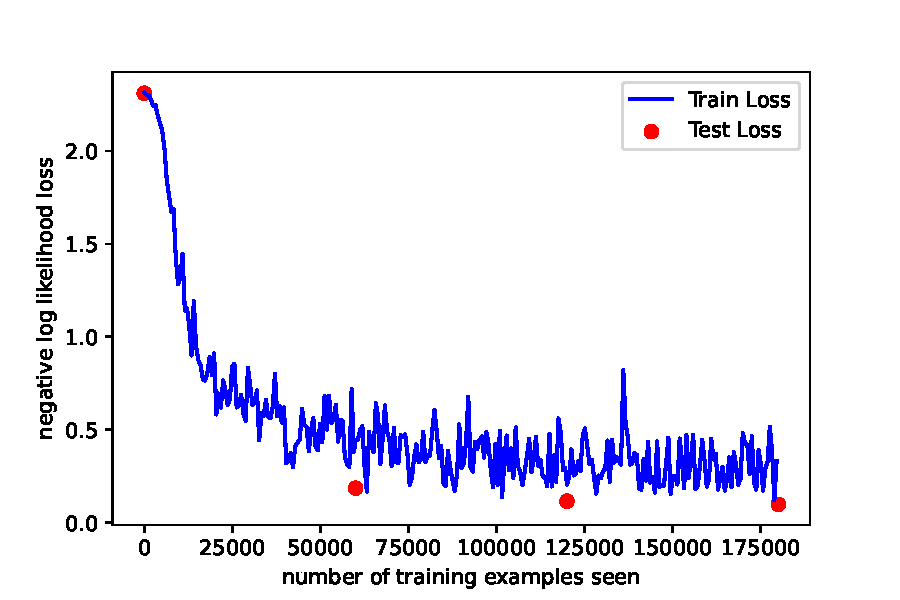
\includegraphics[width=.7\textwidth]{figures/nn-mnist-loss-train.pdf}
\end{center}
\end{frame}



%------------------------------------------------
\begin{frame}{The Vanishing Gradient}

\begin{exampleblock}{}
\begin{itemize}
\item Notice that $\phi'$ is a term in the front of the local gradient, which are multiplied by other local gradients.
\item If the nonlinear activation function saturates then we might run into issues if we're multiplying a bunch on numbers on $(-1,1)$
\end{itemize}
\end{exampleblock}

\uncover<2->{
\begin{tblock}{The Derivative of the Logistic Function}
\begin{multiequation}
\frac{\d}{\d x}\left\{\frac{1}{1+\e^{-x}}\right\}
&= \frac{\uncover<3->{1-1+}\e^{-x}}{(1+\e^{-x})^2}
\uncover<4->{=\frac{1 + \e^{-x}}{(1 + \e^{-x})^2} - \frac{1}{(1 + \e^{-x})^2} }
 \\
\uncover<5->{&= \phi(x)(1-\phi(x)) \leq \frac{1}{4} }
\end{multiequation}
\end{tblock}
}

\end{frame}


%------------------------------------------------
\begin{frame}{The Sigmoid}

\begin{center}
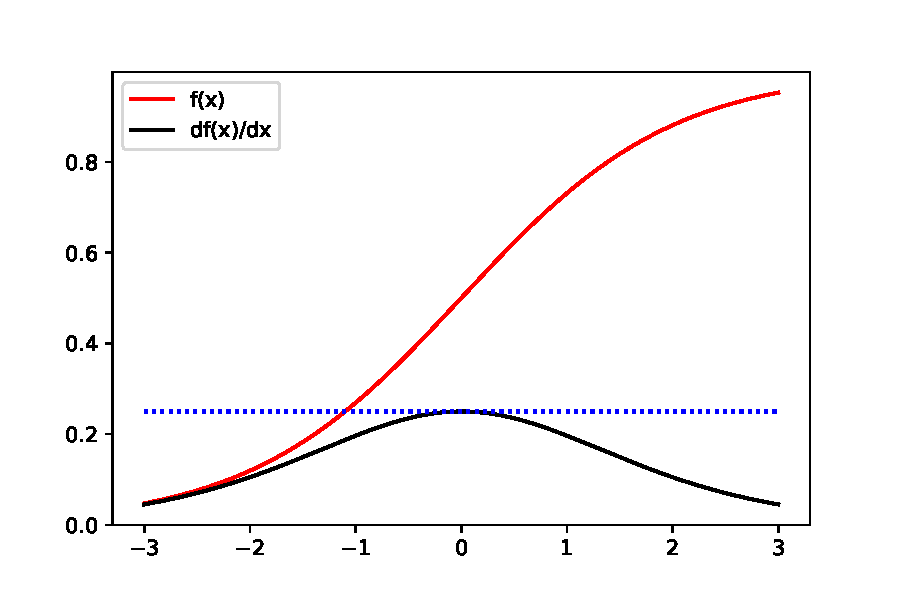
\includegraphics[width=.6\textwidth]{figures/nn-sigmoid.pdf} 
\\
The function $f(x)$ is a sigmoid. The derivative has a maximum value of $1/4$. 
\end{center}
    
\end{frame}



%------------------------------------------------
\begin{frame}{Consequences of the Vanishing Gradient}
\begin{itemize}
    \item The multiplication of the local gradients (and ones coming from the previous layer) can cause the gradient to effectively vanish by the time the updates are done at layers close to the input. 
    \begin{itemize}
        \item Using backpropagation alone is not enough to train a deep multilayer perceptron. We're going to need a different view of training {\em deep neural network} with an MLP. 
        \item Relu-like activation functions can help; however, changing the activation function is not going to be sufficient to {\em effectively} train a deep net. 
    \end{itemize}
    \item Future lectures cover how to effectively train deep nets, but the main take away here is that backpropagation works well at training shallow nets; however, not deep nets. 
\end{itemize}
\end{frame}



%------------------------------------------------
\begin{frame}{Tips to Training Networks}

\begin{tblock}{}
\begin{itemize}
    \item The inputs of your data should be scaled appropriately (e.g., normalization, standardization, etc.)
    \item Outputs of a classification net should be encoded as one-hot vectors; however, we can use {\em sparse representation} and {\em sparse cross-entropy} to avoid directly converting to one-hot.
    \item Training a net is a nonconvex task so different initialization of the weights will lead to different nets. 
    \item Choosing the ``right'' number of layers and nodes at a layer is a {\em heuristic} process. Use the homework as an opportunity to gain experience with the sensitivity of a net to these parameters 
\end{itemize}
\end{tblock}

\end{frame}

\begin{frame}{Tips to Training Networks}
	\begin{block}{}
		\begin{itemize}
			\item On choosing the learning rate: too large, too small, just right\ldots
			\begin{multiequation}
				\eta_{\text{opt}} = \left( \frac{\partial^2 E}{\partial w^2}\right)^{-1} % = \Hbf^{-1}
			\end{multiequation}
			In practice, this terms is tedious to compute every step. 
			\item Anneal the learning rate over time. Choose a larger $\eta$ initially then reduce the value of $\eta$ as the epochs increase
			\item Use early stopping by monitoring the validation error. If the validation error goes up after $k$ successive increases in the loss then stop! 
			\item There is more to put in this slide but you're going to need to get some practice to learn these challenges. 
		\end{itemize}
	\end{block}

\end{frame}



%------------------------------------------------
\begin{frame}{Remember Regularization?}
  {\small\bf\color{MediumBlue}Bishop (2006)}
  Estimation for $\ell^1$-norm (left) and $\ell^2$-norm (right) regularization on 
  $\wbf$. We see the contours of the error function and the regularization constraint 
  on $\|\wbf\|_1 \leq \tau$ and $\|\wbf\|_2^2 \leq \tau^2$.

\end{frame}

%------------------------------------------------
\begin{frame}{Dropout}

\begin{tblock}{Dropout: A new way to regularize a network}
\begin{itemize}
    \item The central idea behind {\em\color{MediumBlue}dropout} is to randomly dropout nodes in the neural network with a probability $p$. After the nodes are ``dropped out'' the remain network is a subnetwork of the original. 
    \item Dropout has been shown to work quite well at preventing overfitting and allowing the network to find a good local minimum. 
    \item {\bf\color{MediumRed}Recommendation}: Use dropout! 
\end{itemize}
\end{tblock}
{\footnotesize
Nitish Srivastava, Geoffrey Hinton, Alex Krizhevsky, Ilya Sutskever, Ruslan Salakhutdinov, ``Dropout: A Simple Way to Prevent Neural Networks from Overfitting,'' {\em Journal of Machine Learning Research}, 15(56):1929--1958, 2014.}
\end{frame}


%------------------------------------------------
\begin{frame}{Dropout in a Neural Network}

\begin{center}
    
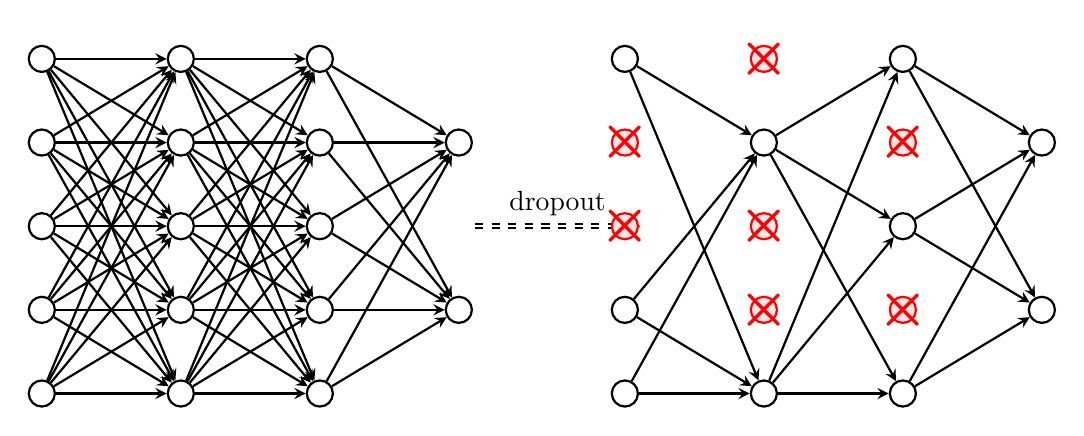
\begin{tikzpicture}

	\node[circle, draw, thick] (i1) {};
	\node[circle, draw, thick, above=2em of i1] (i2) {};
	\node[circle, draw, thick, above=2em of i2] (i3) {};
	\node[circle, draw, thick, below=2em of i1] (i4) {};
	\node[circle, draw, thick, below=2em of i4] (i5) {};
	
	\node[circle, draw, thick, right=4em of i1] (h1) {};
	\node[circle, draw, thick, right=4em of i2] (h2) {};
	\node[circle, draw, thick, right=4em of i3] (h3) {};
	\node[circle, draw, thick, right=4em of i4] (h4) {};
	\node[circle, draw, thick, right=4em of i5] (h5) {};
	
	\node[circle, draw, thick, right=4em of h1] (hh1) {};
	\node[circle, draw, thick, right=4em of h2] (hh2) {};
	\node[circle, draw, thick, right=4em of h3] (hh3) {};
	\node[circle, draw, thick, right=4em of h4] (hh4) {};
	\node[circle, draw, thick, right=4em of h5] (hh5) {};
	
	\node[circle, draw, thick, right=4em of hh2] (o1) {};
	\node[circle, draw, thick, right=4em of hh4] (o2) {};
	
	\draw[-stealth, thick] (i1) -- (h1);
	\draw[-stealth, thick] (i1) -- (h2);
	\draw[-stealth, thick] (i1) -- (h3);
	\draw[-stealth, thick] (i1) -- (h4);
	\draw[-stealth, thick] (i1) -- (h5);
	\draw[-stealth, thick] (i2) -- (h1);
	\draw[-stealth, thick] (i2) -- (h2);
	\draw[-stealth, thick] (i2) -- (h3);
	\draw[-stealth, thick] (i2) -- (h4);
	\draw[-stealth, thick] (i2) -- (h5);
	\draw[-stealth, thick] (i3) -- (h1);
	\draw[-stealth, thick] (i3) -- (h2);
	\draw[-stealth, thick] (i3) -- (h3);
	\draw[-stealth, thick] (i3) -- (h4);
	\draw[-stealth, thick] (i3) -- (h5);
	\draw[-stealth, thick] (i4) -- (h1);
	\draw[-stealth, thick] (i4) -- (h2);
	\draw[-stealth, thick] (i4) -- (h3);
	\draw[-stealth, thick] (i4) -- (h4);
	\draw[-stealth, thick] (i4) -- (h5);
	\draw[-stealth, thick] (i5) -- (h1);
	\draw[-stealth, thick] (i5) -- (h2);
	\draw[-stealth, thick] (i5) -- (h3);
	\draw[-stealth, thick] (i5) -- (h4);
	\draw[-stealth, thick] (i5) -- (h5);
	
	\draw[-stealth, thick] (h1) -- (hh1);
	\draw[-stealth, thick] (h1) -- (hh2);
	\draw[-stealth, thick] (h1) -- (hh3);
	\draw[-stealth, thick] (h1) -- (hh4);
	\draw[-stealth, thick] (h1) -- (hh5);
	\draw[-stealth, thick] (h2) -- (hh1);
	\draw[-stealth, thick] (h2) -- (hh2);
	\draw[-stealth, thick] (h2) -- (hh3);
	\draw[-stealth, thick] (h2) -- (hh4);
	\draw[-stealth, thick] (h2) -- (hh5);
	\draw[-stealth, thick] (h3) -- (hh1);
	\draw[-stealth, thick] (h3) -- (hh2);
	\draw[-stealth, thick] (h3) -- (hh3);
	\draw[-stealth, thick] (h3) -- (hh4);
	\draw[-stealth, thick] (h3) -- (hh5);
	\draw[-stealth, thick] (h4) -- (hh1);
	\draw[-stealth, thick] (h4) -- (hh2);
	\draw[-stealth, thick] (h4) -- (hh3);
	\draw[-stealth, thick] (h4) -- (hh4);
	\draw[-stealth, thick] (h4) -- (hh5);
	\draw[-stealth, thick] (h5) -- (hh1);
	\draw[-stealth, thick] (h5) -- (hh2);
	\draw[-stealth, thick] (h5) -- (hh3);
	\draw[-stealth, thick] (h5) -- (hh4);
	\draw[-stealth, thick] (h5) -- (hh5);
	
	
	\draw[-stealth, thick] (hh1) -- (o1);
	\draw[-stealth, thick] (hh1) -- (o2);
	\draw[-stealth, thick] (hh2) -- (o1);
	\draw[-stealth, thick] (hh2) -- (o2);
	\draw[-stealth, thick] (hh3) -- (o1);
	\draw[-stealth, thick] (hh3) -- (o2);
	\draw[-stealth, thick] (hh4) -- (o1);
	\draw[-stealth, thick] (hh4) -- (o2);
	\draw[-stealth, thick] (hh5) -- (o1);
	\draw[-stealth, thick] (hh5) -- (o2);
	
	\draw[-stealth, double, dashed, thick] (5.5,0) -- node[above] {dropout} (7.6, 0);
	
	
	%%% BOUNDARY %%%
	
	\node[circle, draw, thick, red, fill=red!10, right=10em of hh1] (i1) {};
	\node[circle, draw, thick, red, fill=red!10, above=2em of i1] (i2) {};
	\node[circle, draw, thick, above=2em of i2] (i3) {};
	\node[circle, draw, thick, below=2em of i1] (i4) {};
	\node[circle, draw, thick, below=2em of i4] (i5) {};
	
	\node[red] (icr) at (i1) {$\mathlarger{\mathlarger{\mathlarger{\mathlarger{\mathlarger{\bm{\times}}}}}}$};
	\node[red] (icr) at (i2) {$\mathlarger{\mathlarger{\mathlarger{\mathlarger{\mathlarger{\bm{\times}}}}}}$};
	
	\node[circle, draw, thick, red, fill=red!10, right=4em of i1] (h1) {};
	\node[circle, draw, thick, right=4em of i2] (h2) {};
	\node[circle, draw, thick, red, fill=red!10, right=4em of i3] (h3) {};
	\node[circle, draw, thick, red, fill=red!10, right=4em of i4] (h4) {};
	\node[circle, draw, thick, right=4em of i5] (h5) {};
	
	\node[red] (icr) at (h1) {$\mathlarger{\mathlarger{\mathlarger{\mathlarger{\mathlarger{\bm{\times}}}}}}$};
	\node[red] (icr) at (h3) {$\mathlarger{\mathlarger{\mathlarger{\mathlarger{\mathlarger{\bm{\times}}}}}}$};
	\node[red] (icr) at (h4) {$\mathlarger{\mathlarger{\mathlarger{\mathlarger{\mathlarger{\bm{\times}}}}}}$};
	
	\node[circle, draw, thick, right=4em of h1] (hh1) {};
	\node[circle, draw, thick, red, fill=red!10, right=4em of h2] (hh2) {};
	\node[circle, draw, thick, right=4em of h3] (hh3) {};
	\node[circle, draw, thick, red, fill=red!10, right=4em of h4] (hh4) {};
	\node[circle, draw, thick, right=4em of h5] (hh5) {};
	
	\node[red] (icr) at (hh2) {$\mathlarger{\mathlarger{\mathlarger{\mathlarger{\mathlarger{\bm{\times}}}}}}$};
	\node[red] (icr) at (hh4) {$\mathlarger{\mathlarger{\mathlarger{\mathlarger{\mathlarger{\bm{\times}}}}}}$};
	
	\node[circle, draw, thick, right=4em of hh2] (o1) {};
	\node[circle, draw, thick, right=4em of hh4] (o2) {};
	
	\draw[-stealth, thick] (i3) -- (h2);
	\draw[-stealth, thick] (i3) -- (h5);
	\draw[-stealth, thick] (i4) -- (h2);
	\draw[-stealth, thick] (i4) -- (h5);
	\draw[-stealth, thick] (i5) -- (h2);
	\draw[-stealth, thick] (i5) -- (h5);
	
	\draw[-stealth, thick] (h2) -- (hh1);
	\draw[-stealth, thick] (h2) -- (hh3);
	\draw[-stealth, thick] (h2) -- (hh5);
	\draw[-stealth, thick] (h5) -- (hh1);
	\draw[-stealth, thick] (h5) -- (hh3);
	\draw[-stealth, thick] (h5) -- (hh5);
	
	\draw[-stealth, thick] (hh1) -- (o1);
	\draw[-stealth, thick] (hh1) -- (o2);
	\draw[-stealth, thick] (hh3) -- (o1);
	\draw[-stealth, thick] (hh3) -- (o2);
	\draw[-stealth, thick] (hh5) -- (o1);
	\draw[-stealth, thick] (hh5) -- (o2);

\end{tikzpicture}



\end{center}

\end{frame}
    
      %------------------------------------------------
    
    \begin{frame}[containsverbatim]{Python Notebook}
    \begin{center}
    \small
    { \color{Red}{\url{https://github.com/rahulbhadani/CPE486586_FA26/blob/master/Code/CPE486586_Ch13_Neural_Network.ipynb}}}
    \end{center}
    \end{frame}
    
    %------------------------------------------------
    
    \begin{frame}
        \Huge{\centerline{\color{MediumBlue}\textbf{The End}}}
    \end{frame}

\end{document}